\documentclass{article}

\usepackage{cmlgc}
\usepackage{enumitem}
\usepackage{graphicx}
\usepackage{geometry}
\geometry{
    a4paper
}
\usepackage{hyperref}
\hypersetup{
    colorlinks=true,
    linkcolor=blue,
    urlcolor=blue
}
 
\begin{document}
\newgeometry{
    top=8mm,
    bottom=8mm,
    left=3mm,
    right=8mm
}
\begin{minipage}{0.8\textwidth}
\begin{flushleft}
    \begin{minipage}{1\textwidth}
        \begin{minipage}{.5\textwidth}
            \vspace{.2cm}
            {\huge \textbf{Vadim \textsc{Bertrand}}}\\[.3 cm]
            \url{https://github.com/vadmbertr/}
        \end{minipage}
        \begin{minipage}{.5\textwidth}
        \begin{flushright}
            \begin{minipage}{.74\textwidth}
            \begin{flushright}
                \href{tel:33614623218}{+33 6 14 62 32 18} \\[.1 cm]
                \href{mailto:vadim.bertrand@gmail.com}{vadim.bertrand@gmail.com} \\[.1 cm]
                Grenoble area \\[.1 cm]
                FRANCE
            \end{flushright}
            \end{minipage}
            \begin{minipage}{.24\textwidth}
            \begin{flushright}
                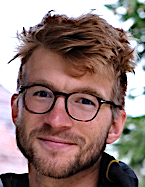
\includegraphics[width=1\textwidth]{picture.png}
            \end{flushright}
            \end{minipage}
        \end{flushright}
        \end{minipage}
    \end{minipage}
    \\[.3 cm]
    \textbf{Statistics and Data Sciences 2\textsuperscript{nd} year Master Student – Software Engineer}
    \\[.5 cm]
    \section*{\textsc{Education}}
    \begin{itemize}
        \item \textbf{2022 – 2023 (expected) \qquad Université Grenoble Alpes – IM\textsuperscript{2}AG} \\
        2\textsuperscript{nd} year Master’s in Statistics and Data Sciences – Labelled “Core IA” by MIAI
        \vspace{-.15cm}
        \begin{itemize}[leftmargin=*]
        \setlength\itemsep{.01cm}
            \item Non-parametric and functional estimation
            \item Computational and High Dimensionality Statistics
            \item Supervised learning: random forest, Support-Vector Machine, Neural Networks
            \item Mathematical optimization
            \item Text mining: MLP, LSTM, Transformers, BERT...
        \end{itemize}
        \item \textbf{2021 – 2022\qquad \qquad \qquad \qquad Université Grenoble Alpes – IM\textsuperscript{2}AG} \\
        1\textsuperscript{st} year Master’s in Statistics and Data Sciences – Labelled “Core IA” by MIAI
        \vspace{-.15cm}
        \begin{itemize}[leftmargin=*]
        \setlength\itemsep{.01cm}
            \item Probability, inferential statistics and statistical tests
            \item Data analysis (PCA, FCA, FCMA)
            \item Linear and Generalized Linear Models
            \item Unsupervised (hclust, k-means, ...) and supervised (k-NN, LDA/QDA, lasso/ridge, ...) learning
            \item Time series analysis
        \end{itemize}
        \item \textbf{2014 – 2015\qquad \qquad \qquad \qquad Université Grenoble Alpes – IAE} \\
        Master’s in Management, specialty Business Administration
        \item \textbf{2011 – 2014\qquad \qquad \qquad \qquad Grenoble INP – Phelma / Ensimag} \\
        Engineering degree “Internet, Services and Connected Systems”
        \vspace{-.15cm}
        \begin{itemize}[leftmargin=*]
        \setlength\itemsep{.01cm}
            \item Database Management System
            \item Distributed systems and applications
            \item Algorithmic
        \end{itemize}
    \end{itemize}
    \section*{\textsc{Professional Experience}}
    \begin{itemize}
        \item \textbf{May. 2022 – Aug. 2022 \qquad Research Internship – DAO team of LJK – Grenoble} \\
        “Deep generative learning for next-generation drugs” – 1\textsuperscript{st} year Master’s internship – \textbf{\textit{ \hyperlink{https://vadmbertr.github.io/Deep-generative-learning-for-next-generation-drugs/Internship_report___Deep_generative_learning_for_next_generation_drugs.pdf}{report}}}
        \vspace{-.15cm}
        \begin{itemize}[leftmargin=*]
        \setlength\itemsep{.01cm}
            \item Extended a 2D image inpainting CNN to 3D and drugs generation tasks
            \item Used an invariant ligand-protein complex representation based on oriented residue density grids
            \item Implemented using PyTorch library
        \end{itemize}
        \item \textbf{Sept. 2016 – Aug. 2021 \qquad Engineer – DANCE team (CNRS / Inria) – Grenoble}
        \vspace{-.15cm}
        \begin{itemize}[leftmargin=*]
        \setlength\itemsep{.01cm}
            \item Developed, deployed and maintained applications for collecting, estimating and predicting road traffic indicators in real time in the Grenoble Metropolis via the use of models designed by members of the team
            \vspace{-.15cm}
            \begin{itemize}[leftmargin=*]
            \setlength\itemsep{.01cm}
                \item \url{http://gtl.inrialpes.fr} (stable) \\
                Pre-processing – filtering and imputation – estimates and predictions using MATLAB
                \item \url{http://gtlville.inrialpes.fr} (experimental)
                \vspace{-.15cm}
                \begin{itemize}[leftmargin=*]
                \setlength\itemsep{.01cm}
                    \item Developed mostly using the Python ecosystem
                    \item Collects data from multiple heterogeneous sources
                    \item Relies on NetworkX, pandas and xarray for datasets manipulations
                    \item Handles spatial data through Shapely, PyGEOS and OpenLR
                    \item Backed by a PostgreSQL relational database and PostGIS extension
                \end{itemize}
            \end{itemize}
            \item Collaborated with PhD / post-doctoral students and supervised interns
                \vspace{-.15cm}
                \begin{itemize}[leftmargin=*]
                \setlength\itemsep{.01cm}
                    \item Evaluated the impact of reducing the maximum speed limit to 70kmph on pollutant emissions on Grenoble’s south ring during pollution peaks
                    \item Built a dynamic partition model – based on nodes’ state – of a road network to estimate travel times through the obtained partitions – \textbf{\textit{\hyperlink{https://hal.archives-ouvertes.fr/hal-01953560}{paper}}}
                \end{itemize}
            \item Wrote technical documentation for the opening of a public tender to collect traffic data
        \end{itemize}
    \end{itemize}
\end{flushleft}
\end{minipage}
\hfill\vline\hfill
\begin{minipage}{0.15\textwidth}
    \begin{minipage}{1\textwidth}
    \begin{flushleft}
        \textbf{1994} \\
        First snowplows \\[.2cm]
        \textbf{1996} \\
        Judo white belt \\[.2cm]
        \textbf{1998} \\
        Initiation to rugby \\[.9cm]
        \textbf{2007} \\
        Sport-study rugby program \\[.5cm]
        \textbf{2012} \\
        3 months in Australia \\[.2cm]
        \textbf{2014} \\
        Switch to ski touring \\[.1cm]
        \textbf{2015} \\
        2 months around the Balkans \\[.2cm]
        \textbf{2017} \\
        Transition to Touch rugby \\[.2cm]
        \textbf{2019} \\
        Rediscovered chess \\[.1cm]
        \textbf{2020} \\
        1\textsuperscript{st} diving level \\[.1cm]
        \textbf{2021} \\
        Integrated the M30 Touch rugby French selection
    \end{flushleft}
    \end{minipage}
    \begin{minipage}{1\textwidth}
    \vspace{7.9cm}
    \begin{flushleft}
        \textbf{Languages} \\[.1cm]
        English \quad Fluent \\
        Spanish \quad Notions
    \end{flushleft}
    \end{minipage}
    \begin{minipage}{1\textwidth}
    \vspace{1cm}
    \begin{flushleft}
        \textbf{Miscellaneous} \\[.1cm]
        Python, C++, R \\
        \LaTeX \\
        Git \\
        Docker \\
        Shell scripting \\
        QGIS software
    \end{flushleft}
    \end{minipage}
\begin{flushleft}
    
\end{flushleft}
\end{minipage}

\end{document}
